%%% Methods Section
\section{Methods}

In the case of the mono energic point source the source is directly surrounded by HDPE, as shown in Figure ~\ref{fig:PointSrcGeo}. 
The \iso[252]{Cf} source is not presented as a bare point source.
Rather, the source is modeled as as a point \iso[252]{Cf} source sournded by 0.5 cm of lead. The lead sphere is then encased in HDPE as shown in Figure ~\ref{fig:Cf252SrcGeo}.
In both source configurations the source is taken to be isotropic. 
For the point source was modeled for neutron energies of 1 eV, 1 keV, and 1 MeV.
The \iso[252]{Cf} source was modeled using the spontanous fission spectra built into MCNPX.
\begin{figure}
  \centering
  \begin{subfigure}[b]{0.45\textwidth}
    \centering
    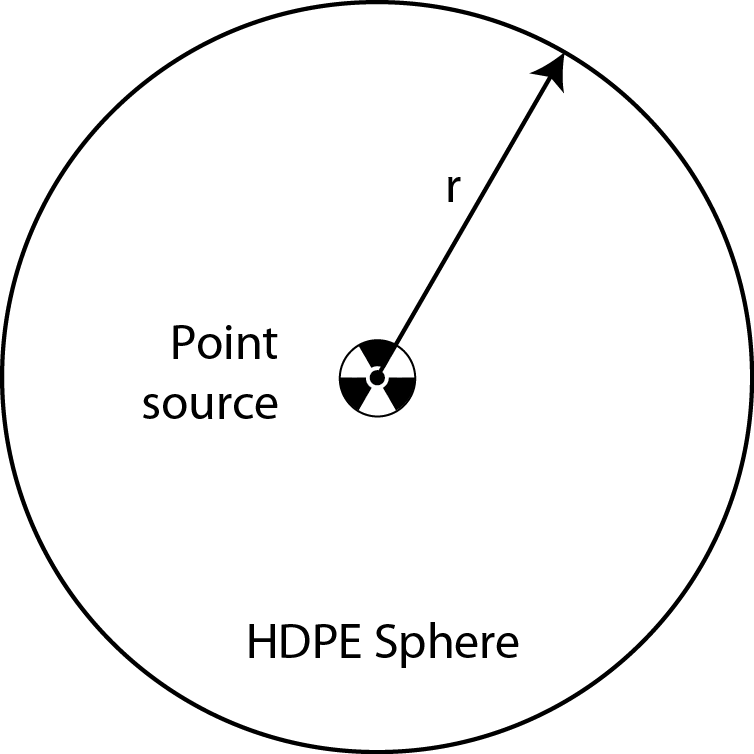
\includegraphics[width=\textwidth]{HDPEModeration_PointSrcGeo}
    \caption{Geometry of mono energetic point source}
    \label{fig:Cf252SrcGeo}
  \end{subfigure}%
  ~
  \begin{subfigure}[b]{0.45\textwidth}
    \centering
    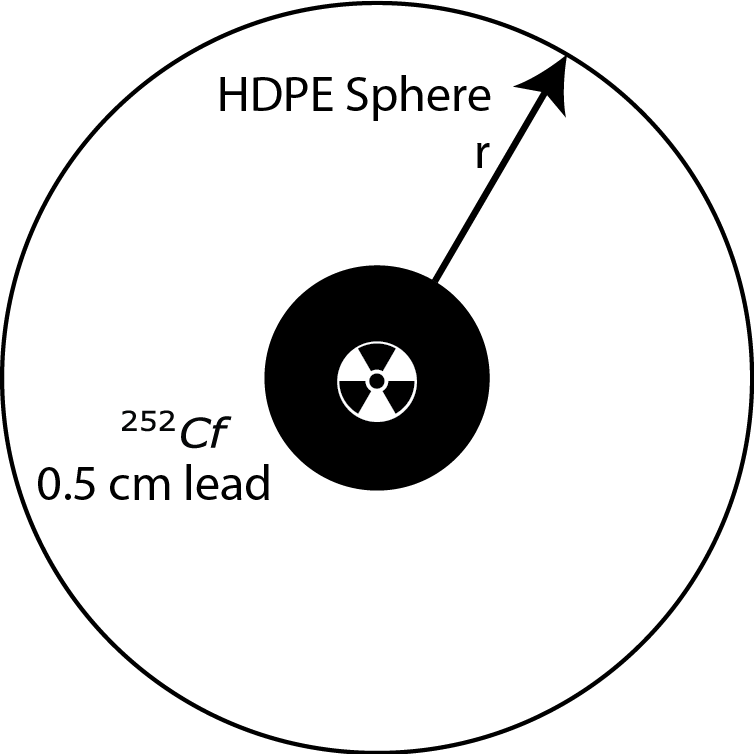
\includegraphics[width=\textwidth]{HDPEModeration_Cf252SrcGeo}
    \caption{Geometry of \isotope[252]{Cf} source}
    \label{fig:Cf252SrcGeo}
  \end{subfigure}
  \caption{Simulated Geometry}
\end{figure}

The thermal fraction is defined in \eqref{eqn:ThermalFraction} and was calculated by bining into two energy bins seperated by $5\times10^{-7}\text{MeV}$ (0.5 eV), normalizing by the total flux.
The thermal energy of 0.5 eV was chosen because this is the close to the cadmium cutoff.
\begin{align}
    \label{eqn:ThermalFraction}
    \eta = \frac{\int_0^E_\text{termal} \phi(E)dE}{\int_0^\infty \phi(E)dE}
\end{align}

\subsection{Simulation}
%%%%%%%%%%%%%%%%%%%%%%%%% LISTING CODE %%%%%%%%%%%%%%%%%%%%%%%%%%
%\lstinputlisting[linerange={217-220},caption=World Physical Volume,label=lst:World]{src/DetectorConstruction.cc}
